\documentclass[letterpaper,12pt]{article}
\usepackage[utf8]{inputenc}
\usepackage{fullpage}
\usepackage{courier}
\usepackage[margin=0.75in]{geometry}
\usepackage{listings}
\usepackage{color}
\usepackage{graphicx}
\usepackage[width=5in]{caption}
\usepackage{hyphenat}
\usepackage[section]{placeins}

% Format a sectionless paragraph
\newcommand*\unparagraph{
	\par
	\nopagebreak
	\vskip3.25ex plus1ex minus.2ex
	\noindent
}

% define extra colors
\definecolor{dkgreen}{rgb}{0,0.6,0}
\definecolor{purple}{RGB}{159,0,197}

% define the code listing format
\lstset{
	language=C++,
	basicstyle=\footnotesize\ttfamily,
	backgroundcolor=\color{white},
	showspaces=false,
	showstringspaces=false,
	frame=none,
	tabsize=3,
	keywordstyle=\color{purple},
	commentstyle=\color{dkgreen},
	stringstyle=\color{blue},
	escapeinside={\%*}{*)}
}

% define the title/header
\title{\Large CS 1428 Honors\\Lab 1} 
\author{Jared Wallace}
\date{}

\begin{document}

\maketitle

\vspace{30mm}

\section*{Questions}
Throughout the semester, we will be building a program piece by piece.
This program that you will be writing will function as an \emph{assembler},
which means that it will in turn run other, much smaller and much more basic, programs.
I will be writing and giving to you those small, basic programs for your assembler to run.
Today we will start writing the assembler. To facilitate the modular approach we are taking with
this project, we are going to maintain it in a \emph{Git} repository.

The initial setup for a git repository is fairly straightforward. For the purposes of this class,
I'm going to just give you the steps with a minimal explanation. For more information, see the link
on the website or just ask me during office hours. Go ahead and pull up a terminal window, either by
booting Linux or by opening PuTTy and connecting to Eros (I'll explain how). Then follow these steps:
\begin{enumerate}
    \item mkdir Lab\_Files
    \item cd Lab\_Files
    \item mkdir Assembler
    \item cd Assembler
    \item touch README.md
    \item git init
    \item git add README.md
    \item git commit -m 'Initial'
    \item ssh-keygen -t rsa (press enter for each prompt)
    \item cat .ssh/id\_rsa.pub
    \item stop and wait for instructions to setup a remote repository
    \item git config --global user.name "your\_name\_here"
    \item git config --global user.email "your\_email\_here"
    \item git push origin master
\end{enumerate}

Now, when you write the program for last item of this lab, you will "save" your work by doing:
\begin{enumerate}
    \item git add //name of file//
    \item git commit -m 'Enter a witty commit message here'
    \item git push origin master
\end{enumerate}

\begin{enumerate}
    \item(10 pts) Every C++ program starts out with the same basic form, or skeleton.
         What are the different parts of this skeleton?
         What is the name of the function that all C++ functions must include?
    \vspace{40mm}
    \item(10 pts) Evaluate the following expressions.
         Write the answers on this work sheet (You may show your work for partial credit).
         Do \emph{not} use the computer to evaluate these expressions.
         \begin{enumerate}
             \item 10 \% 456
             \item 12 \% 3
             \item 16 \% 5
             \item 0 \% 456
         \end{enumerate}
    \item (10 pts) Evaluate the following expressions exactly as the computer would evaluate them.
          (You may show your work for partial credit). Do \emph{not} use the computer to evaluate
          these expressions. Be sure and account for floating point vs. integer division \emph{and}
          order of operations!
            \begin{enumerate}
                \item 12 / 2 - 4
                \item 7 / 3
                \item 6.0 / 4
                \item (6 + 17) \% 2 - 1
                \item 14 / (11 / 4)
            \end{enumerate}
    \item (10 pts) Consider the following C++ snippet:
            \begin{lstlisting}
                int cars = 10;
                int trucks = 2;
                int busses = 1;
                int vans = 5;
                int count = 2;

                cars += busses;
                trucks += trucks + busses;
                busses += 3;
                ++busses;
                vans = vans/ count;
            \end{lstlisting}
            \begin{table}[h!]
            \begin{center}
                \begin{tabular}{|c|c|c|c|c|c|}
                    \hline
                    step & cars & trucks & busses & vans & count \\ \hline
                    1 & & & & & \\ \hline
                    2 & & & & & \\ \hline
                    3 & & & & & \\ \hline
                    4 & & & & & \\ \hline
                    5 & & & & & \\ \hline
                \end{tabular}
            \end{center}
            \end{table}
            After execution, what are the values of the following variables? (Hint: use the table)

            cars:

            trucks:

            busses:

            vans:
    \item (10 pts) The mini-programs I give you will use simple integers to represent various
          commands the program you write can execute. For instance, the number 0 will mean “add”.
          Each instruction line in the mini-program will have 3 extra integer values (representing the data
          for the matching command) along with it.
          How do you declare 4 integer variables named inst, data0, data1, and data2?
          How would you declare an additional string variable named source?
    \vspace{40mm}
    \item (5 pts) How would you set the value of inst to 0, data0 to 5, data1 to 4, and data2 to 2?
    \vspace{40mm}
    \item (10 pts) How would you assign the sum, difference, product, modulo, and quotient
          of data1 and data2 to the variable named data0? (Do each assignment as a separate statement)
    \vspace{40mm}
    \item (10 pts) Let’s decide that we wanted to use named constants to represent the various
          commands our program can execute. Declare the following named constants with the given values:
          (All are integer constants)
            \begin{itemize}
                \item OP\_ADD with a value of 0
                \item OP\_SUB with a value of 1
                \item OP\_MUL with a value of 2
                \item OP\_DIV with a value of 3
                \item OP\_MOD with a value of 4
                \item OP\_EXP with a value of 5
                \item OP\_RED with a value of 6
                \item OP\_WRT with a value of 7
            \end{itemize}

    \item (25 pts) You will need to make a program named lab1h.cpp that combines what you have done
          in questions 1 through 5. Requirements:
            \begin{itemize}
                \item Make sure you have the proper header and includes
                \item Make sure you have the 'using namespace' compiler directive and a 'main' function.
                \item At the top of your main function, include the named constants you declared in question 5.
                \item Inside your main function, you will need to declare the 4 integer variables
                      you wrote in question 2. You will also need to prompt the user for the values of
                      each variable, and then store the value they input into the appropriate variable.
                \item You will also need to perform the 5 calculations in question 4, and after performing
                      each one, output the result of the calculation to the screen on its own line.
                \item Ensure that your program compiles \emph{and} produces correct output.
            \end{itemize}
\end{enumerate}
\section*{Deliverables}
Hard copy of the source code you wrote (assembler.cpp) and the answers to the questions.
Soft copy (upload to homework upload) of your source code.

% Comic at the bottom
\begin{figure}[ht!]
	\centering
	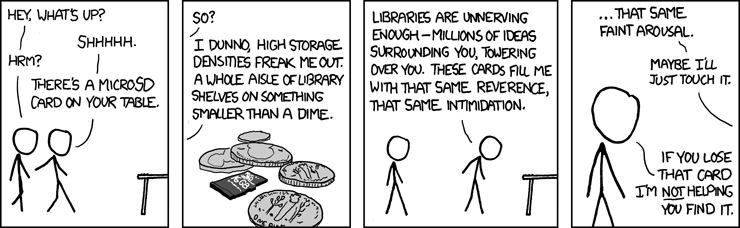
\includegraphics[width=5in]{microsd.png}
\caption*{That card holds a refrigerator carton's worth of floppy discs, and a soda can full
          of those cards could hold the entire iTunes store's music library. Mmmm.}
\end{figure}
\end{document}
